%% LyX 2.3.6.2 created this file.  For more info, see http://www.lyx.org/.
%% Do not edit unless you really know what you are doing.
\documentclass[english]{report}
\usepackage{mathptmx}
\usepackage{helvet}
\usepackage{courier}
\usepackage[T1]{fontenc}
\usepackage[latin9]{inputenc}
\usepackage{fancyhdr}
\pagestyle{fancy}
\usepackage{verbatim}
\usepackage{graphicx}

\makeatletter

%%%%%%%%%%%%%%%%%%%%%%%%%%%%%% LyX specific LaTeX commands.
%% Because html converters don't know tabularnewline
\providecommand{\tabularnewline}{\\}

%%%%%%%%%%%%%%%%%%%%%%%%%%%%%% User specified LaTeX commands.
\usepackage{lastpage} 
\renewcommand{\headrulewidth}{0.4pt} 
\renewcommand{\footrulewidth}{0.4pt} 
\lhead{\$-SiteId}
\chead{page \thepage \space of \pageref{LastPage}}
\lfoot{\$-SiteOperator}
\cfoot{\today}
\rhead{Period:\$-MoniPeriod}
\rfoot{\$-Author}

\makeatother

\usepackage{babel}
\begin{document}

\section*{Monitoring of Storage Unit in the Grid Structure}
\noindent \begin{center}
\begin{tabular}{ll}
SITE : & \$-SiteId \tabularnewline
OPERATOR : & \$-SiteOperator \tabularnewline
MONITORING PERIOD : & \$- MoniPeriod \tabularnewline
EVALUATION DATE : & \$-EvaDate\tabularnewline
\end{tabular}
\par\end{center}

\subsection*{Introduction}

This report provides analysis and presentation of measured data for
the storage system

\$-SiteId

SiteDescription 

The storage unit is located at

It enables installation and operation of an enlarged PV-Generator
with 2.5 times higher peak power by means of buffering PV generation,
ensuring the line power to stay within the limits allowed. 

-

\noindent The report is conforming with the EC Guidelines for unified
monitoring and performance assessment of storage-units in the grid
structure. 

\noindent Thus, it reveals energy balancing in a subgrid, characterized
by both energy surplus and autonomy ratio. Further it quantifies and
details contribution of the storage unit to grid control and balancing,
and thus relief of the utility interface, resp. power line. 

\noindent In the form of directed power-flows, monitoring data is
suitable for spatial aggregation with results from other storage units
in a common grid area. 

\noindent Further to reporting for storage and distribution system
operators, guideline conformant data and monitoring evaluation qualify
for sharing performance experience, e.g. in the JRC's storage observatory.

\subsection*{General Data}

\begin{tabular}{lll}
Storage Unit & Nominal Power/{[}MW{]}: \$-NomStoPow & \multicolumn{1}{l}{Nominal Capacity/{[}MWh{]}: \$-NomStoCap}\tabularnewline
Utility Interface & Nominal Power/{[}MW{]}: \$-NomUIPPow  & Site : \$-SiteId\tabularnewline
\end{tabular}

\newpage

\subsection*{Energetic Balances }

In line with recording format from independent metering, the total
energies in the monitoring period sum up to :\vspace{0.3cm}

\begin{tabular}{lrlrl}
 & ~~~~~~~~Input &  & ~~~~~~~~Output & \tabularnewline
Subgrid & 17.5 & MWh & 19.5 & MWh\tabularnewline
Utility & 30.0 & MWh & 30.0 & MWh\tabularnewline
Storage & 28.0 & MWh & 25.0 & MWh\tabularnewline
\end{tabular}	 

\vspace{0.3cm}

\noindent with the total difference between in- and outputs covering
the storage losses.

\noindent In accumulation of directed powerflows, the energy exchanges
of the storage unit with subgrid surpluses(net generation) and deficits(net-load),
and with the utility can be distinguished from the direct flows between
subgrid and utility.\vspace{0.3cm}

\begin{tabular}{lrl}
net-generation to utility & ~~~~~~~~19.58 & MWh\tabularnewline
storage from net-generation & 25.00 & MWh\tabularnewline
storage from utility & 3.21 & MWh\tabularnewline
storage to utility & 2.73 & MWh\tabularnewline
storage to net-load & 25.07 & MWh\tabularnewline
net-load from utility & 30.84 & MWh\tabularnewline
\end{tabular}\vspace{0.3cm}


\subsection*{Exchange Yields}

Normalizing the directed powerflows, to the nominal power of the storage
unit, is resulting in yields, comparable for units of different sizes.
Chart 1 shows the exchange yields in their daily averages .\vspace{0.3cm}

\noindent \begin{center}
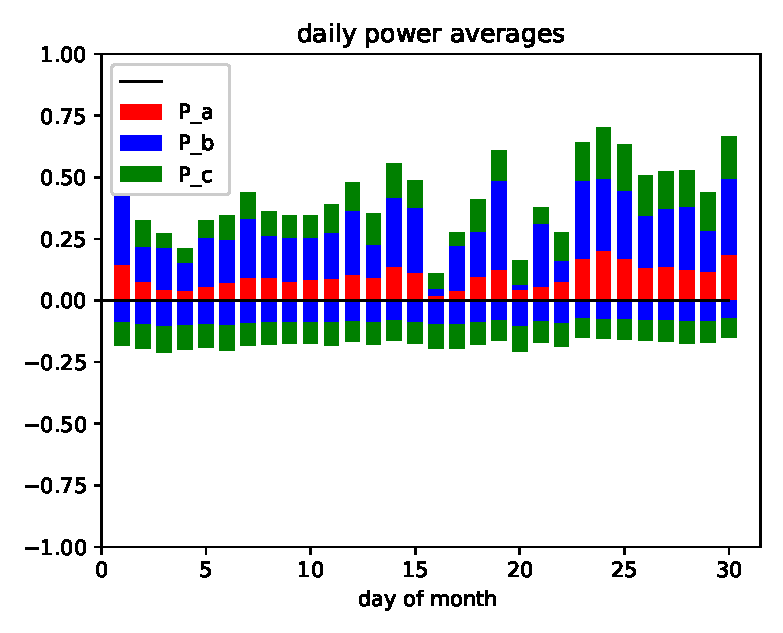
\includegraphics[scale=0.52]{Image_chart1}
\par\end{center}

\begin{center}
chart 1 : Average DailyYields
\par\end{center}

\newpage{}

\noindent Accordingly chart 2 shows the hourly averages of the exchange
yields, reflecting average operation in the daily course. \vspace{0.3cm}

\begin{center}
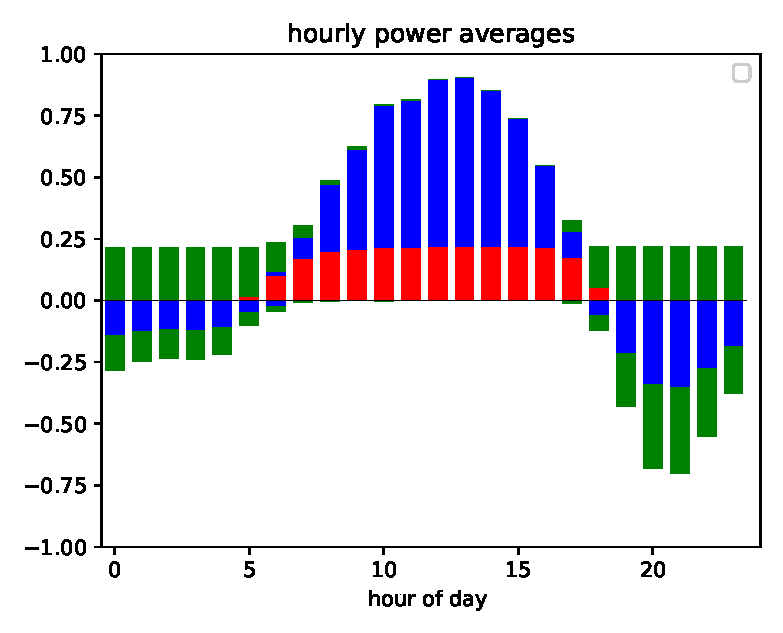
\includegraphics[scale=0.55]{Image_chart2}
\par\end{center}

\vspace{0.3cm}

\begin{center}
chart 2 : Average HourlyYields
\par\end{center}

\subsection*{Storage Performance in the Grid }

Performance is resulting from average yields in the monitoring period,
indicating the contribution of the storage unit to balancing. control.
This compares to the total balancing need of the subgrid and the remaining
balancing control, required from the utility interface.\vspace{0.3cm}

\textbf{Subgrid Yields}

\begin{tabular}{clcccc}
Input : & \_\_\_~~~~~~~~~ & Output : & \_\_\_ & Balance Depth : & 10.5 hrs\tabularnewline
\end{tabular}

\textbf{Utility Yields}

\begin{tabular}{clcccc}
Input : & ~~~~~~~~~\_\_\_ & Output : & \_\_\_ & Balance Depth : & 17.0 hrs\tabularnewline
\end{tabular}

\textbf{Storage Yields}

\begin{tabular}{llcccc}
Input : & ~~\_\_\_ & Throughput : & \_\_\_ & Balance Depth : & 23.0 hrs\tabularnewline
\multicolumn{3}{l}{Subgrid Balancing} & \_\_\_ &  & 20.5 hrs\tabularnewline
\multicolumn{3}{l}{Shifted Generation} & \_\_\_ &  & 2.0 hrs\tabularnewline
\multicolumn{3}{l}{Shifted Load Coverage} &  &  & 0.5 hrs\tabularnewline
\end{tabular}

\vspace{0.3cm}

\noindent Operation of the storage unit in time-shift of generation
surplus, resp. of load deficit, is separated from operation in balancing
the subgrid generation surplus with its load deficit. Time-shift operation
reflects operation control performance and includes all exchanges
with the utility interface, as well as planned services as unplanned.
The storage usage and the longterm energetic losses are characterized
by 

\noindent \vspace{0.3cm}

\noindent %
\begin{tabular}{llll}
Recharge Ratio : & 112 \% & Equivalent Full-Cycles : & 120\tabularnewline
\end{tabular}\newpage{}

\subsection*{Utility Interface Relief}

Further resolving the balancing needs over increasing timespans, resp.
balancing periods, results in the Balance Duration Curve of throughput,
and the corresponding capacity as integral over the periods, visible
as area under the curves. \vspace{0.3cm}

\begin{center}
\includegraphics[scale=0.6]{Image_fig1}
\par\end{center}

\vspace{0.3cm}

\begin{center}
figure 1 : Yields vs Balance-Durations before and behind Storage
\par\end{center}

\begin{comment}
Time shift operation plus two curves positive deficit load shift from
grid together with negative surplus generation shift to grid
\end{comment}

\noindent With the balancing yields of the subgrid in red, storage
is balancing net-power yields over the red area for the balancing
capacity employed, the normalized balance depth in {[}hrs{]}. The
residual utility balance duration curve in blue remains to be compensated
by the outer grid infrastructure., with the blue area for the total
balancing depth required.

\noindent Complementary to the energetic balancing, the effect of
storage unit operation on releasing the grid interface from power
amplitude is quantified. This graph reveals how storage operation
is modifying the characteristics of normalized power yields. For the
subgrid yields in red, allocated storage is releasing the utility
interface, which then covers the blue part only.\vspace{0.3cm}

\begin{center}
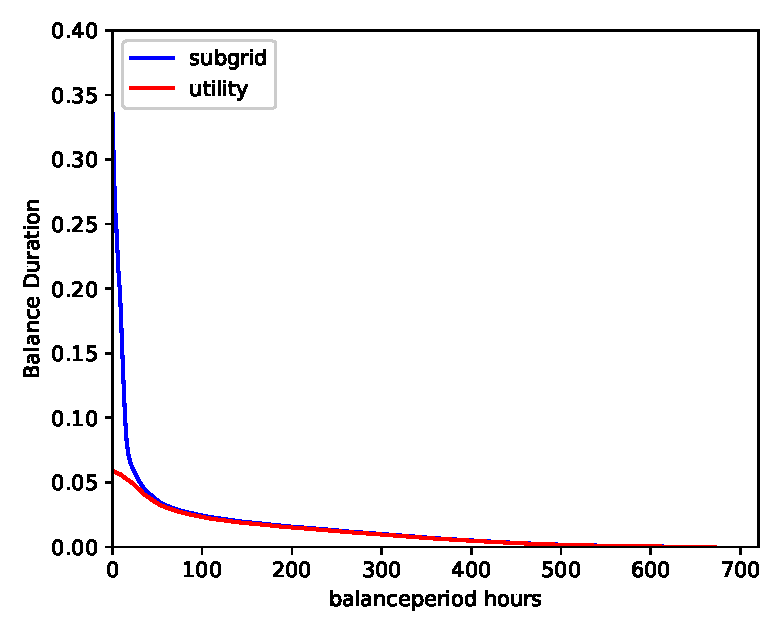
\includegraphics[scale=0.6]{Image_fig2}
\par\end{center}

\vspace{0.3cm}

\begin{center}
figure 2 : Yields vs Power-Durations before and behind Storage
\par\end{center}

\subsection*{\newpage}

\subsection*{Subgrid Coverage Performance Ratios}

In relation to the average net load yield $\bar{Y}_{NL}$ in the monitoring
period, subgrid coverage is characterized by performance ratios. Storage
and utility are covering the total net load of the subgrid \vspace{0.3cm}

\begin{tabular}{cccc}
 & Net-Surplus Ratio & Throughput Ratio & Net-Load Coverage \tabularnewline
\textbf{Subgrid} & 120 \%  & 100 \% & 21 hrs\tabularnewline
Utility & 50 \% & 30 \% & 14.5 hrs\tabularnewline
Storage & 70 \% & 70 \% & 6.5 hrs\tabularnewline
\end{tabular}

\vspace{0.3cm}


\subsection*{Annuities}

Based on storage unit power cost of :- PowCost -: Euro per MW-: ,
and capacity\_cost of :- CapCost -: Euro per MWh on a financing term
of :- FinTerm -: years and :- OpEx -:\% operation costs, the annuities
are resulting as: \vspace{0.3cm}

\begin{tabular}{cccc}
Total expenditure annuity & power~~~ & capacity  & operation\tabularnewline
23 Euro/MWh & 32\% & 60\% & 8\%\tabularnewline
\end{tabular}\newpage
\end{document}
